\documentclass[10pt]{article}


\usepackage[a4paper , left=31.7mm, top=25.4mm]{geometry}


\usepackage{hyperref}
\hypersetup{
	colorlinks=true,
    linkcolor=blue,
    filecolor=magenta,      
    urlcolor=cyan,
    pdftitle={Overleaf Example}
}

\setlength\parindent{0pt}
\usepackage{listings}
% Copyright 2017 Sergei Tikhomirov, MIT License
% https://github.com/s-tikhomirov/solidity-latex-highlighting/

\usepackage{listings, xcolor}

\definecolor{verylightgray}{rgb}{.97,.97,.97}

\lstdefinelanguage{Solidity}{
	keywords=[1]{anonymous, assembly, assert, balance, break, call, callcode, case, catch, class, constant, continue, constructor, contract, debugger, default, delegatecall, delete, do, else, emit, event, experimental, export, external, false, finally, for, function, gas, if, implements, import, in, indexed, instanceof, interface, internal, is, length, library, log0, log1, log2, log3, log4, memory, modifier, new, payable, pragma, private, protected, public, pure, push, require, return, returns, revert, selfdestruct, send, solidity, storage, struct, suicide, super, switch, then, this, throw, transfer, true, try, typeof, using, value, view, while, with, addmod, ecrecover, keccak256, mulmod, ripemd160, sha256, sha3}, % generic keywords including crypto operations
	keywordstyle=[1]\color{blue}\bfseries,
	keywords=[2]{address, bool, byte, bytes, bytes1, bytes2, bytes3, bytes4, bytes5, bytes6, bytes7, bytes8, bytes9, bytes10, bytes11, bytes12, bytes13, bytes14, bytes15, bytes16, bytes17, bytes18, bytes19, bytes20, bytes21, bytes22, bytes23, bytes24, bytes25, bytes26, bytes27, bytes28, bytes29, bytes30, bytes31, bytes32, enum, int, int8, int16, int24, int32, int40, int48, int56, int64, int72, int80, int88, int96, int104, int112, int120, int128, int136, int144, int152, int160, int168, int176, int184, int192, int200, int208, int216, int224, int232, int240, int248, int256, mapping, string, uint, uint8, uint16, uint24, uint32, uint40, uint48, uint56, uint64, uint72, uint80, uint88, uint96, uint104, uint112, uint120, uint128, uint136, uint144, uint152, uint160, uint168, uint176, uint184, uint192, uint200, uint208, uint216, uint224, uint232, uint240, uint248, uint256, var, void, ether, finney, szabo, wei, days, hours, minutes, seconds, weeks, years},	% types; money and time units
	keywordstyle=[2]\color{teal}\bfseries,
	keywords=[3]{block, blockhash, coinbase, difficulty, gaslimit, number, timestamp, msg, data, gas, sender, sig, value, now, tx, gasprice, origin},	% environment variables
	keywordstyle=[3]\color{violet}\bfseries,
	identifierstyle=\color{black},
	sensitive=false,
	comment=[l]{//},
	morecomment=[s]{/*}{*/},
	commentstyle=\color{gray}\ttfamily,
	stringstyle=\color{red}\ttfamily,
	morestring=[b]',
	morestring=[b]"
}

\lstset{
	language=Solidity,
	backgroundcolor=\color{verylightgray},
	extendedchars=true,
	basicstyle=\footnotesize\ttfamily,
	showstringspaces=false,
	showspaces=false,
	numbers=left,
	numberstyle=\footnotesize,
	numbersep=9pt,
	tabsize=2,
	breaklines=true,
	showtabs=false,
	captionpos=b
}

\usepackage{tikz}
\newlength{\Lnote}
\newcommand{\notte}[1]
     {\addtolength{\leftmargini}{1em}
        \settowidth{\Lnote}{\textbf{Note:~}}
        \begin{quote}
            \rule{\dimexpr\textwidth-2\leftmargini}{1pt}\\
                        \mbox{}\hspace{-\Lnote}\textbf{Note:~}%
                                            #1\\[-0.5ex] 
            \rule{\dimexpr\textwidth-2\leftmargini}{1pt}
        \end{quote}
        \addtolength{\leftmargini}{-4em}}
\graphicspath{ {./assets/images/} }








\title{Viral-Next Gen Social Communication Tool}
\date{15 January 2022}
\author{Joby Reuben\\jobyreuben@gmail.com}



\begin{document}




\maketitle

\section{Abstract}
This is a Sample Abstract of the Viral Project.

\section{User Problems \& Basic Solutions}
This is a Sample Problems of the Viral Project.

\section{Vision Statement}
To bring blockchain \& crypto adoption to the masses we would got to bridge social communication with defi and tokenised economy. The Viral Network of Applications standards are designed in such a way that our vision to bring an proficient, user-friendly mobile application will combine several divisions of decentralized protocols that can lead to an ultimate tool for crypto acknowledgement. The divisions which we are focussing to rebuild is listed\\
\\
\textbf{\large Social Media}
\begin{enumerate}
\item To create a Real-world Decentralised Social Media
\item To construct an Autonomous self-evolving platform
\item To construct an Interactive Next-Gen Social Media
To form a clean people-owned platform appropriate for all age groups
\end{enumerate}
\textbf{\large Crypto Adoption}
\begin{enumerate}
\item To provide people to hop into crypto from fiat effortlessly \& securely
\item To give access to use cryptocurrencies to internet people without investing
\item To bring all major crypto for individuals to adapt rapidly using a single wallet
\end{enumerate}
\textbf{\large NFT \& Metaverse}
\begin{enumerate}
\item To democratize NFTs to Masses
\item To kickstart Metaverse adoption
\end{enumerate}
\textbf{\large Blockchain}
\begin{enumerate}
\item To supply the utmost speed of transactions through On-Chain \& Off-Chain solutions
\item To Develop a feeless, fast, Zero Inflation, Deflationary, smart contract chain
\end{enumerate}
\newpage
	\tableofcontents

\newpage
\section{Unified Mobile Application - An Intro to Viral}

\hyperlink{https://sample.com}{App Brouchure}\\

\textit{Images}\\

A Next-Gen Social Media platform bridging interactive media, NFTs, and blockchain technologies' underlying applications into an every-day user-based mobile app. Viral bridges Social Media with Blockchain, Wallets, Exchanges and NFT Markeplaces to bring the ultimate one-app for the common masses to adopt into the tokenised economy.\\

Every media shared on viral is an unique NFT where it can be utilized to create limitless achievable outcomes across the platform. Users can share ultra-short to short videos, thoughts through text, sell NFTs and additionally make communication between one-on-one, private groups and, open channels with total genuine privacy. App users will be benefitted from zero ads, cryptographic encryption, censorship-resistant and, also get to use various cryptocurrencies throughout the platform. Every user is an active contributor to the platform by which they receive rewards (payment) in Viral Coin for effectively utilizing the Viral Application and it's child platforms.\\

\section{Viral Platform Architecture}

\textit{Diagram}\\

\begin{enumerate}

\item \textbf{Viral App}: Decentralized Social Media Platform bridging Blockchain applications for limitless possibilities.

\item \textbf{Viral Smart Chains}: Horizontally Scalable EVM Smart Chain on Top of IOTA's Tangle.

\begin{enumerate}

	\item \textbf{Payment Channels (L2)}: State Channels to move value off-chain for lightning fast micro-transactions.

	\item \textbf{Zk-Rollups (L2)}: Batching Multiple Off-chain NFT Standard Tokens (ERC721) to On-Chain,
	\item \textbf{Viral Bridge}: Interopability of various major cryotocurrencies by wrapping tokens decentralized such as Bitcoin, Ethereum,etc into Viral Smart Chains.
	\item \textbf{Horizontal Chains}: Additional of New Chains anchored to IOTA Tangle that communicates between multiple Viral Smart Chains for unlimited scaling

\end{enumerate}

\item \textbf{Smart Wallet}: Viral's App's built in Non-Custodial Viral Smart Chain compatible hot wallet that allows user to send \& hold tokens, mint NFTs and receive rewards.

\begin{enumerate}

\item \textbf{Viral CEX-Centralized Exchange}: Trustless Non-Custodial Exchange for Fiat-Crypto trading
\item \textbf{Viral DEX-Decentralized Exchange}: Automated Market Making Protocol for exchanging Viral tokens
\item \textbf{P2P Exchange}: Trustsless anonymous exchange leveraging Peer-to-Peer protocol
\item \textbf{Viral Name System}: Decentralized blockchain based username protocol for transfers instead of cryptographic public address.

\end{enumerate}

\item \textbf{Child Platforms}: Independant platforms anchored to the viral network for effective improvement of protocols

\begin{enumerate}

\item \textbf{Dev-Space}: Application for Developers to decide on reward allocation for improving Viral-Beta
\item \textbf{ROV App}: Curator Platform to vote and remove reported content on Viral-Alpha
\item \textbf{Ad Platform}: Decentralized Ad platform connecting Influencers,businesses and users for trustless engagement-proof ads.
\item \textbf{Reward Pool}: To incentivize all users, miners, developers using smart contracts for their content, validation of transactions, and continuous development through unbiased pointing strategy that offers more rewards to bigger contributors.

\end{enumerate}

\item \textbf{Other Backend}: For contingencies which will be later decentralized in the further phases of the development roadmap

	

\end{enumerate}

	\subsection{Development Tech Stack}

	\textit{Diagram}\\

	\begin{enumerate}

	\item \hyperlink{https://ipfs.io}{IPFS}: IPFS stands for Interplanetary File System is a peer-to-peer distributed file system that is used for maintaining and distributing files across our Viral IPFS Private network.

	\item \hyperlink{https://gun.eco/}{GunDB}: GunDB is a fully decentralized graph database to store information from user to user meaning that your changes are not affected by any centralized server.

	\item \hyperlink{https://webrtc.org/}{WebRTC}: WebRTC stands for Web Real-Time Communication, an open-source project built primarily for peer-to-peer real-time connections.

	\item \hyperlink{https://www.javascript.com/}{Javascript}: JavaScript is a text-based programming language used both on the client-side and server-side that allows you to make web pages interactive.

	\item \hyperlink{https://nodejs.org/}{NodeJS}: Node.js is an open-source, cross-platform, back-end JavaScript runtime environment that runs on the V8 engine and executes JavaScript code outside a web browser.

	\item \hyperlink{https://reactjs.org/}{ReactJS}: React is a free and open-source front-end JavaScript library for building user interfaces based on UI components.

	\item \hyperlink{https://docs.soliditylang.org/}{Solidity}:Solidity is an object-oriented, high-level language for implementing smart contracts, mostly used for executing code in Ethereum Virtual Machine

	\item \hyperlink{https://wiki.iota.org/smart-contracts/overview}{IOTA Smart Contract Protocol}: The IOTA ecosystem allows to spin up a smart contract blockchain and anchor it to the IOTA tangle
	
	\end{enumerate}


\section{How Whitepaper Structured}
For an efficient understanding, we have seperated the Viral Architecture/Ecosystem's major sectors.\\

\begin{itemize}
\item Social Media \& User Experience (Page 1-10)
\item Blockchain, Token Ecosystem \& Layer 2 (Page 10-15)
\item Smart Wallet (Page 15-20)
\item Child Platforms (Page 20-25)
\item Revenue \& Incentives (Page 25-30)
\item Viral DAO  \& Governance
\end{itemize}

\section{Social media \& User Experience}
Viral is a multi-media sharing decentralized social network that brings meta-experience with friends, family and other people to communicate, share posts and send messages across the globe with absolute privacy. Viral sets Non-Fungible-Tokens (NFT) as a standard for every post that shared in the network which intends to bring interactive social experience and utility use cases of blockchain environment.\\

\notte{To bring NFT as a standard for a social media post doesn't essentially implies it ought to be sold for tokens, rather it conveys that each post in Viral is a unique piece of data in the blockchain that gives the power of ownership of the user which if needed can be opted to transfer in exchange for tokens inside the Viral Platform.\texttt{notte}.}

\begin{lstlisting}[language=Solidity, caption={NFT Snippet for Enable/Disable Open Sale}]

pragma solidity ^0.8.10;

contract HelloWorld {

    string public greet = "Hello World!";
    
}
\end{lstlisting}

\subsection{Types of Post}
\hyperlink{https://sample.com}{ELI5 Explanatory Video - Viral NFTs}\\

Please read \hyperlink{App Brouchure}{https://sampel.com/} to have a visual experience of the Viral Social Network\\

\textit{Image for all Post Types in a Visualized Manner}

\subsubsection{Shots}

Shots are \textbf{10 sec motion pictures} with added loop transitions to bring life to photos. Pictures can be shared as shots, an exciting looped motion picture.\\

People can share their
\begin{enumerate}
\item Personal Sneak-Peek, Moments \& Events
\item Exclusive Photoshoots, commercials, to your fans
\item Turn photos into lively shots by adding shot animations through Viral
\end{enumerate}

\subsubsection{Thoughts}
Thoughts are \textbf{text-based sharing} for micro-blogging. Attach photos, long/short videos, documents, etc. There is no limit on words or media. People can share other users thoughts to their followers using re-Thought feature.

\subsubsection{Drops}
Drops are \textbf{20 second disappearing stories} shared to followers which auto-disappears once seen. It features AR filters, texts, shot elements, links, music, transitions and, much more. Every Drops will be purged in 30 days\\

\notte{Drops will not be minted as unique NFT due to it's nature of disappearing media\texttt{notte}.}

\subsubsection{Interactive Videos}
IVs are short 30sec full-screen\textbf{narration based videos}. It is based on\textbf{gamification of videos} to interact within the videos.

\subsubsection{NFT Utilities}
Minting (Creating) an NFT in Viral is\textbf{as easy as creating a social media post}. Viral provides multiple NFT utilities for users to mint, buy, sell with an easy user experience.

Viral will take a\textbf{1.5\% commission} selling NFTs which will be reverted to the reward pool

\subsubsection{Tunes}

Artists can\textbf{sell their music albums}, singles as NFT for the fans/people to buy and own it

\begin{lstlisting}[language=Solidity, caption={NFT Snippet To Sell Multiple Copies}]

pragma solidity ^0.8.10;

contract HelloWorld {

    string public greet = "Hello World!";
    
}
\end{lstlisting}

\subsubsection{Sketch}
\textbf{Digital arts}, paintings, sketches can be sold through NFTs

\begin{lstlisting}[language=Solidity,label={single-asset}, caption={NFT Snippet to sell single asset}]

pragma solidity ^0.8.10;

contract HelloWorld {

    string public greet = "Hello World!";
    
}
\end{lstlisting}

\subsubsection{Originals}
\textbf{Physical assets} can be sold through Viral's Original NFTs where people can buy and flex

\begin{lstlisting}[language=Solidity, caption={NFT Snippet to provide extra information such as Name, Address, Mobile Number, before transferring coins with end to end encryption between seller}]

pragma solidity ^0.8.10;

contract HelloWorld {

    string public greet = "Hello World!";
    
}
\end{lstlisting}

\subsubsection{Tickets}
\textbf{Exclusive passes} for events, ownership of clubs, a digital ticket for everything can be sold as NFT. See Listing \ref{single-asset}

\subsubsection{Filters}
Filters can be sold, and owned by user's thereby get rewards for it

\begin{lstlisting}[language=Solidity, caption={NFT Snippet to distribute shares Just like company share where if 100 NFTs is sold, the person who holds 50 NFT will hold 50\% of the company}]

pragma solidity ^0.8.10;

contract HelloWorld {

    string public greet = "Hello World!";
    
}
\end{lstlisting}

Please read \hyperlink{App Brouchure}{https://sampel.com/} to have a visual experience of the Viral Social Network

\subsection{Avatars}

Personalized Avatars are generated free for every viral user using a selfie. Users can edit their avatar skin, outfit, hair, etc. These avatars will be shown in their public profile where other users can see them 3D View.\\

\textit{Image}\\

These avatars are brought into Viral to integrate metaverse and to provide an \textbf{interactive experience}\\

\hyperlink{Avatar Demo-Video}{https://sampel.com/}\\

\begin{lstlisting}[language=Solidity]

// ReadyPlayerMe Integration Examples

1. ReadyPlayerMe WebView- How creating Avatars work using Partner API
2. Downloading Asset- GLB File using Event Listener
3. Mapping skeletons and face
4. Animating and storing the file as a 3D Viewer File inside the application using IPFS Public/Clusters
5. How Animations will work

\end{lstlisting}

\subsubsection{Meta-Chat}

Meta-Chat is a feature to \textbf{show your facial reactions} in real-time when you chat with your friend. Viral captures your face reactions and transfer it to your avatar which the mutual friend can see on \textbf{top of his/her chat page}.

\textit{Image}\\

This gives you a \textbf{virtual experience} of videocalls through avatars and text chat.

\hyperlink{Meta-Chat Demo}{https://sampel.com/}\\

\textbf{SDKs and APIs Used} : List the APIs\\

\textit{Formula\\
Flowcharts}

\subsubsection{Live \& Rooms}

Decentralized \textbf{Live Video Events and Audio Rooms using Avatars} (or) Normal Cams. Celebrities can host live events with their fans using their avatars\\

\textit{Image}\\
\hyperlink{Live-Events Demo}{https://sampel.com/}\\
\textbf{SDKs and APIs Used} : List the APIs\\

\textit{Formula\\
Flowcharts}

\subsection{Engagements}

\textbf{Like, Comment, Share, Tip}\\

Users can like, comment, share, reThought, and also tip Tokens to their favorite posts and influencers. The number of likes will influence the recommendations list of other users.\\

Additionally a hidden engagement dislike will be added to every post but won't be visible to the users/nor owners, which is exclusively utilized for interest-based algorithm to filter out disliked content\\

\textit{Algorithm/Mathematical formula for recommendation engine}\\

\textbf{Tip}\\

The tipping feature in Viral engagements tip/support user's favourite influencers' contents. It works as a donation/reward where all the tips will be directly sent to the receivers wallet. Users can send tokens of their own choice to reward other users content on the platform.

Viral will charge commisions on Tips and deposits it to the reward pool. These commissions are calculated in such a way where the percentage varies depending on the end face value.\\

The tipping amount will be round of to tens and will leave the commision on both seperated amounts.\\

$Formula$\\

The Charges are\\


(Ending with 1,2)\$ tips     - 22\%      i.e., 11, 62, 761, 952\\
(Ending with 3,4,5)\$ tips   - 19\%      i.e., 23, 64, 765, 953\\
(Ending with 6,7,8,9)\$ tips - 17\%      i.e., 16, 48, 27,  79\\
(Ending with 0)\$ tips       - 12\%      i.e., 10, 60, 720, 1000\\


For example: If a user is tips worth 57\$ then the commissions charged will be:\\

For the first     50\$ - 12\%\\
And the remaining 7\$  - 17\%\\
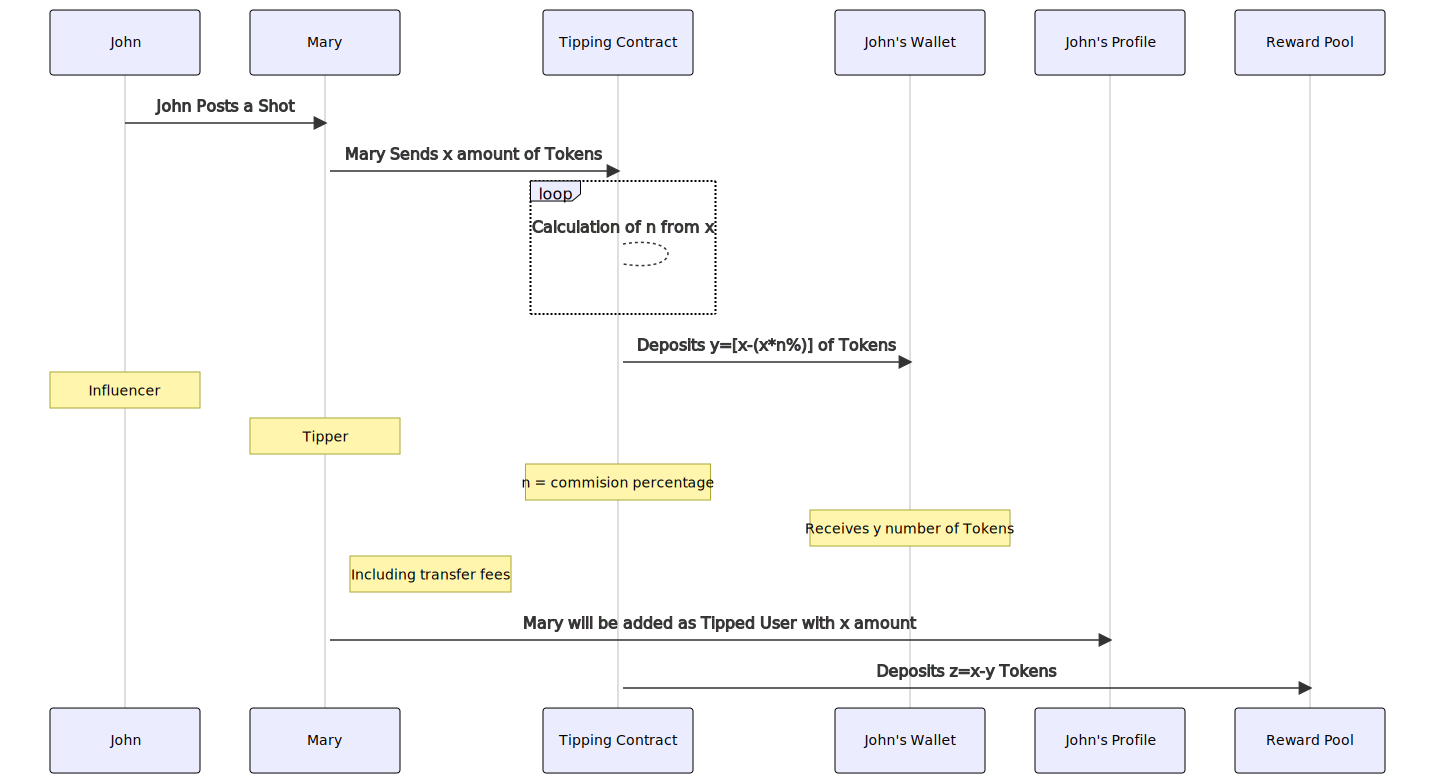
\includegraphics[width=\textwidth]{tips}\\

\begin{lstlisting}[language=Solidity, caption={Tipping Solidity Snippet}]

pragma solidity ^0.8.10;

contract HelloWorld {

    string public greet = "Hello World!";
    
}

\end{lstlisting}

\subsection{Other Features}

\subsubsection{Privacy Groups}

Privacy Groups is a unique feature in Viral to create unlimited friend's groups list to ensure maximum privacy for users to post and share to particular groups of users i.e., Family, Friends, Close Friends, Besties, etc. This feature can empower complete privacy over viewers for certain posts.

































\end{document}



